\documentclass[handout]{beamer}
\usepackage{verbatim}
\usepackage{xcolor}
\usepackage{multirow}
\usepackage{amssymb}
\usepackage{tikz}
\usetikzlibrary{positioning,fit}
%\usepackage{enumitem}
\usetheme{Warsaw}
\setbeamertemplate{navigation symbols}{}
\newcommand{\blue}[1]{{\color{blue} #1}}
\newcommand{\red}[1]{{\color{red} #1}}
\newcommand{\grn}[1]{{\color{green} #1}}
\newcommand{\bluRed}[2]{{\color{blue} #1}{\color{red} #2}}
\newcommand{\qtns}[0]{\begin{center} Questions? \end{center}}
\newcommand{\nl}[1]{\vspace{#1 em}}
\newcommand{\cntrImg}[2]{\begin{center}\includegraphics[scale=#2]{#1}\end{center}}
\newcommand{\defn}[1]{{\bf #1}}
\let\emptyset\varnothing
\newcommand{\SampS}[0]{$\mathcal{S}$}

\title{Math 3070, Applied Statistics}

\begin{document}

\begin{frame}
    \begin{beamercolorbox}[rounded=true,wd=\textwidth,center]{title}
        \usebeamerfont{title}\inserttitle
    \end{beamercolorbox}
    \begin{center}
        Section 1\\
        \nl{0.5}
        September 21, 2019
    \end{center}
\end{frame}

\begin{frame}{Lecture Outline, 9/21}
    Section 4.1
    \begin{itemize}
        \item Expected Value and Standard Deviation Revisited
        \item Probability Density Functions
        \item Uniform Random Variables
        \item Examples
    \end{itemize}
\end{frame}

\begin{frame}{Expected Value and Standard Deviation Revisited}
    Suppose that you have a data set $x_i$ where the number 1 shows up $200$ times, the number 2 shows up $300$ times and the number 3 shows up $300$ times. This data set has a $800$ observations.\\ \nl{0.5}
    Let's compute the sample mean.
    $$ \frac{1}{800}\sum_{i=1}^{800} x_i = 1 \blue{\frac{200}{800}} + 2 \blue{\frac{300}{800}} + 3 \blue{\frac{300}{800}}= 2.125$$
    Now compute the expected value of the random variable $X$ with the folowing PMF
    \[
    f(x) = P(X=x) = \left\{\begin{array}{lr}
        2/8, & x=1\\
        3/8, & x=2\\
        3/8, & x=3\\
        0, & \text{otherwise}
        \end{array}\right. \]
        $$ E[X] = 1 \blue{\frac{2}{8}} + 2 \blue{\frac{3}{8}} + 3 \blue{\frac{3}{8}} = = 2.125$$
    \end{frame}

    \begin{frame}{Expected Value and Standard Deviation Revisited}
        In the frequentist view of statistics, the $E[X]$ measures the center or average of a random variable. When sample size increases, the sample mean becomes closer to this theoretical mean which is related to other parameters depending on distribution.
        \end{frame}

        \begin{frame}{Expected Value and Standard Deviation Revisited}
            Suppose that you have a data set $x_i$ where the number 1 shows up $200$ times, the number 2 shows up $300$ times and the number 3 shows up $300$ times. This data set has a $800$ observations.\\ \nl{0.5}
            Let's compute the sample variance.
            $$ \frac{1}{800}\sum_{i=1}^{800} x_i = (1-2.125)^2 \blue{\frac{200}{800}} + (2- 2.125)^2 \blue{\frac{300}{800}} + (3-2.125)^2 \blue{\frac{300}{800}}= 2.125 $$
            
            Each squared term is the distance from the mean or the deviation away from the mean.  

                $$ V(X) = E[(X-E[X])^2] = $$
                $$(1-2.125)^2 \blue{\frac{2}{8}} + (2-2.125)^2 \blue{\frac{3}{8}} + (3-2.125)^2 \blue{\frac{3}{8}} = 2.125 $$
                Both variances measure spread from the mean. In the same way as with the means, the sample variance becomes closer to the theoretical variance.
            \end{frame}

\begin{frame}{Continuous Random Variables}
    So far, we have only discussed discrete random variables, which have only a sequence of possible values (usually whole numbers):
    \begin{itemize}
    \item The number of defective widgets in a batch.
    \item The number of widgets inspected before finding one defective.
    \item The number of customers who visit a store in an hour.
    \end{itemize}
    However, many quantities in real life vary continuously:
    \begin{itemize}
    \item The length of a metal rod.
    \item The strength of a specimen of concrete.
    \item The weight of a bottled drink.
    \item The amount of time until the next customer arrives.
    \end{itemize}
    We will need different techniques to deal with continuous random variables.
    \end{frame}

    \begin{frame}{Continuous Random Variable}
        \begin{block}{}
        We say that a random variable $X$ is \textbf{continuous} if $P(X=x)=0$ for every $x$. If there is a function $f(x)$ such that for all $a\leq b$,
        $$P(a \leq X \leq b) = \int_a^b f(x)\ dx$$
        then we call $f(x)$ a \textbf{probability density function} (pdf) of $X$.
        \end{block}
        
        
        \begin{tabular}{p{5cm}p{4.5cm}}
        \vspace{.4cm} To be a valid pdf, we must have
        \begin{enumerate}
        \item $f(x)\geq 0$ for all $x$.
        \item $\int_{-\infty}^{\infty} f(x)=1$.
        \end{enumerate}
        &
        \vspace{-.55cm}
        \hspace*{-.6cm}
        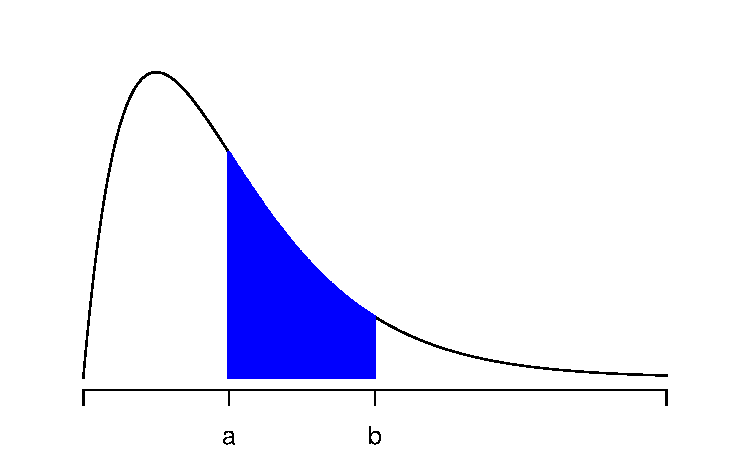
\includegraphics[scale=.55]{ch4_pdf_gam.pdf}
        \end{tabular}
        \end{frame}

        \begin{frame}{Standard Uniform Random Variable}
            Define a pdf by
            $$f(x)=\begin{cases}1 & \text{if }0\leq x\leq 1 \\
            0 & \text{otherwise}\end{cases}$$
            The continuous random variable $X$ with this pdf is called a \textbf{standard uniform} random variable; it takes values uniformly on the interval [0,1]. $X\sim unif(0,1)$
            \begin{tabular}{@{}p{5.5cm}p{4.5cm}}
            \vspace{0cm}For example, the probability that $X$ is between .2 and .6 is
            \begin{center}$\begin{aligned}[t]
            &P(.2 \leq X \leq .6) \\
            &=\int_{.2}^{.6} 1\ dx\\
            &= x\vert_{.2}^{.6}\\
            &= .6-.2\\
            &=.4
            \end{aligned}$\end{center}
            &
            \vspace{0cm}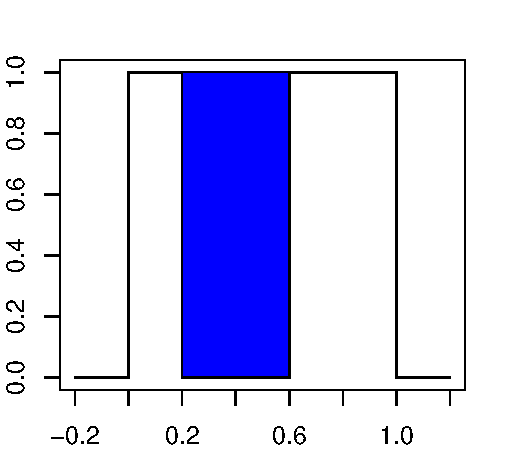
\includegraphics[scale=.6]{ch4_pdf_unif.pdf}
            \end{tabular}
            \end{frame}
            
            \begin{frame}{Uniform Random Variable}
            \begin{block}{}
            We say that $X$ is a \textbf{uniform} random variable on the interval $[a,b]$ if $X$ has pdf
            $$f(x)=\begin{cases}\frac1{b-a} & \text{if }a\leq x\leq b \\
            0 & \text{otherwise}\end{cases}$$
            $X\sim Unif(a,b)$
            \end{block}
            \pause Example: Suppose that the time we have to wait at a bus stop is a uniform random variable $X$ between 0 and 15 minutes. What is the probability that we will have to wait more than 10 minutes?
            \pause \begin{align*}
            P(X\geq 10) &= \int_{10}^\infty f(x)\ dx \\
            &= \int_{10}^{15} \frac1{15-0}\ dx \\
            &= \frac1{15}x\big\vert_{10}^{15} = \frac{15-10}{15} = 1/3
            \end{align*}
            \end{frame}
    \begin{frame}{Summary}
        \begin{itemize}
            \item $X$ is continuous if $P(X=x) =0$ for all $x$.
            \item The probability density function PDF $f$ of $X$ satisfies
            $$ P(a \leq X \leq b) = \int_{a}^b f(x) dx.$$
            This means that the proability of events involving on continuous random variables can be computed used integrals.
            \item Need $f(x)\geq 0$ for all $x$ and $\int_{-\infty}^{\infty} f(x)=1$.
            \item The PDF identifies the continuous random variable.
            \item $X \sim unif(a,b)$ or a random variable $X$ is uniformly distributed on the interval $[a,b]$ means $X$ has 
            $$f(x)=\begin{cases}\frac1{b-a} & \text{if }a\leq x\leq b \\
            0 & \text{otherwise}\end{cases}$$
            as it's PDF. Note, $a,b$ from this bullet point is not the same as the previous $a,b$
        \end{itemize}
    \end{frame}
    \begin{frame}{Example, Non-PDFs}
        Which of the following could be PDFs?
        $$f(x)=\begin{cases} \frac{\cos(x)}{2} & \text{if }0\leq x\leq \pi \\
        0 & \text{otherwise}\end{cases} \hskip 1em g(x)=\begin{cases} \frac{\sin(x)}{2} & \text{if }0\leq x\leq \pi \\
        0 & \text{otherwise}\end{cases}$$
        \pause
        $$ f(3\pi /4) = -1/\sqrt{2} < 0 $$
        $f(x)\geq 0$ is false. $f(x)$ cannot be a PDF.\\ \nl{0.5}
        \pause 
        $g(x) \geq 0$ is true. $g=0$ outisde $[0,\pi]$.
        \pause
        $$\int_{-\infty}^\infty g(x) = \int_{0}^{\pi} \frac{\sin{(x)}}{2} dx = -\frac{\cos{(x)}}{2} \bigg|_{x=0}^\pi = 1$$
        $g(x)$ could be a PDF.\\ \nl{0.5}
        \pause If fact, it is one since the PDF identifies the random variable.
    \end{frame}

    \begin{frame}{Example, Unbounded $X$ and Complement Example}
        Show that 
        $$f(x)=\begin{cases} e^{-x} & \text{if }0\leq x \\
        0 & \text{otherwise}\end{cases} $$
        is a PDF. Compute the probability of $X>1$.\\ \nl{0.5}
        \pause $f(x)\geq 0$ for all x.
        \pause $$ \int_{-\infty}^\infty f(x) dx = \int_{0}^\infty e^{-x} dx = -e^{-x}\bigg|_{x=0}^\infty = 0 - (-1) = 1 $$
        \pause $f(x)$ is a PDF since it satisfies the conditions.
    \end{frame}
    \begin{frame}{Example, Unbounded $X$ and Complement Example}
        Show that 
        $$f(x)=\begin{cases} e^{-x} & \text{if }0\leq x \\
        0 & \text{otherwise}\end{cases} $$
        is a PDF. Compute the probability of $X>1$.\\ \nl{0.5}
        \pause 
        $$ P(X>1) = \int_{x=1}^\infty e^{-x} dx = -e^{-x}\bigg|_{x=1}^\infty = 0 - (-e^{-1}) = e^{-1} $$
        \begin{align*}
            \pause
        P(X>1) &= 1- P(X\leq 1) = 1 - \int_{-\infty}^{1} f(x) dx \\
        & = 1 - \int_{0}^{1} e^{-x} dx =  1 - \bigg( -e^{-x} \bigg|_{x=0}^1\bigg)\\
        & = 1 - \bigg( -e^{-1} +1 \bigg) = e^{-1}
        \end{align*}
    \end{frame}
    \begin{frame}{Example, Unbounded $X$ and Complement Example}
        Show that 
        $$f(x)=\begin{cases} e^{-x} & \text{if }0\leq x \\
        0 & \text{otherwise}\end{cases} $$
        is a PDF. Compute the probability of $X>1$.\\ \nl{0.5}
        The take away is that both work and the laws of probability work the same way.
        \\ \nl{0.5}
        Here's a detail that can be used for continuous random variables.
        $$ P(X\leq 1) = P(X=1) + P(X<1) = 0 + P(X<1) $$
        Here we are breaking up disjoint sets and using the fact that the probability of observing any single value is zero.
    \end{frame}
    \begin{frame}{Example, Another Complement Example}
        For the random variable $X$ which has the follow PMF
        $$f(x)=\begin{cases} \frac{1}{2} e^{-x} & \text{if }0\leq x \\
        \frac{1}{2} e^{x} & \text{if } 0> x \end{cases} $$
        Compute the probability that $0>X$ or $1<X$.
        \\ \nl{0.5}
        \begin{align*}
        \pause \{ 0>X\text{ or } 1<X \}' &=  (\{ 0>X \} \cup \{1<X \})'\\
        \pause & = \{ 0>X \}' \cap \{1<X \}' \\
        & = \{ 0\leq X \} \cap \{1\geq X \} \\
        \pause & = \{ 0\leq X \leq 1\}\\
        \end{align*}
    \end{frame}
    \begin{frame}{Example, Another Complement Example}
        For the random variable $X$ which has the follow PMF
        $$f(x)=\begin{cases} \frac{1}{2} e^{-x} & \text{if }0\leq x \\
        \frac{1}{2} e^{x} & \text{if } 0> x \end{cases} $$
        Compute the probability that $0>X$ or $1<X$.
        \\ \nl{0.5}
        \begin{align*}
            P( 0>X\text{ or } 1<X ) & = 1 - P(0\leq X \leq 1)\\
            \pause & = 1 - \int_{0}^1 f(x)dx = 1 - \int_{0}^1 \frac{1}{2} e^{-x}dx\\
            & = 1 - \frac{1}{2}\bigg( -e^{-x} \bigg|_{x=0}^1 \bigg)\\
            & = 1 - \frac{1}{2}\bigg( -e^{-1} + 1 \bigg) = \frac{1 + e^{-1}}{2}
        \end{align*}
    \end{frame}
    \begin{frame}{Example, Conditioning Example}
        The ratio of served and leftover food is uniformly distributed on the interval $[0,1]$. Compute the probablity that less than a quarter of the of food remains given that half of the food is leftover.
        \\ \nl{0.5}
        \pause
        $X\sim unif(0,1)$
        $$ f(x)=
        \begin{cases} \frac{1}{1-0} & \text{if }0\leq x < 1 \\
        0 & \text{otherwise}\end{cases}
        =
        \begin{cases} 1 & \text{if }0\leq x < 1 \\
        0 & \text{otherwise}\end{cases}
         $$
         \pause
        Condition the event $\{ X<0.25 \}$ on the event $\{ X<0.5 \}$.
         \begin{align*}
            \pause P(X<0.25 | X<0.5) &  = \frac{P(X<0.25,X<0.5)}{P(X<0.5)}\\
           \text{(use containment)} & = \frac{P(X<0.25)}{P(X<0.5)} = \frac{\int_{-\infty}^{0.25} f(x) dx)}{\int_{-\infty}^{0.5} f(x) dx}\\
            & = \frac{\int_{0}^{0.25} 1 dx}{\int_{0}^{0.5} 1 dx}  = \frac{0.25}{0.5} = 0.5\\
         \end{align*}
    \end{frame}
    \begin{frame}{Summary}
        \begin{itemize}
            \item Sets are typically written in terms of inequalities.
            \item Complement and Conditioning work the same way.
            \item Unions and Intersections are useful to know, but, in this class, it is easier to reduce the set to simpler sets. For example:
            $$ \{X<0\} \cup \{X<1\} = \{X<1\} $$
            $$ \{X<0\} \cap \{X<1\} = \{X<0\} $$
        \end{itemize}
    \end{frame}
\end{document}